\documentclass{llncs}
\usepackage{fullpage}

%load needed packages
\usepackage{graphicx}
\usepackage{array}
\usepackage{booktabs}
\usepackage[utf8]{inputenc}
\usepackage{amsmath} 


\begin{document}

\title{APPLICATION OF CLUSTERING METHODS TO
	SPORULATION YEAST MICROARRAY DATA}

\author{Diego De Pablo}
\institute{\email{depablodiego@uma.es} \\
Health Engineering. Málaga University.}

\maketitle 

\vspace{1cm} % Space down the title

\textit{This work presents a comparison between three main clustering methods applied to yeast sporulation data: K-means, hierarchical clustering and self-organizing maps (SOM). K-means was used to cluster genes based on expression patterns, selecting the optimal number of clusters using the elbow method. Hierarchical clustering allowed to analyze the structure of the data without predefining a number of clusters, using a dendrogram to identify significant groups. Finally, SOM was applied as an unsupervised clustering technique, with a visual representation reflecting the topology of the data. This comparison aims to evaluate the effectiveness of each method in gene clustering, similar to the work Comparisons and validation of statistical clustering techniques for microarray gene expression data}

% This is a comment


\section{Introduction}


The aim of this study is to apply clustering techniques to a DNA microarray dataset of \textit{Saccharomyces cerevisiae} gene expression during sporulation, and compare the results with those from a separate analysis.


\subsection*{Temporal Patterns in Gene Expression During Sporulation}

Gene expression during sporulation follows distinct temporal patterns, observe the figure \ref{fig:Sporlutation}, reflecting specific cellular events \cite{chu1998}. These include:
\begin{itemize}
	\item \textbf{Metabolic Early:} Rapid induction at t0.
	\item \textbf{Early I and II:} Sustained expression from t0.5 to t2.
	\item \textbf{Early-Middle:} Peak expression around t5.
	\item \textbf{Middle:} Activation between t5 and t7, related to meiosis.
	\item \textbf{Mid-Late:} Increased expression from t7 to t9, linked to spore wall formation.
	\item \textbf{Late:} Induction between t9 and t11.5, associated with spore maturation.
\end{itemize}
\vspace{-25pt}

\begin{figure}[h!]
	\begin{center}  % Usamos el entorno 'center'
		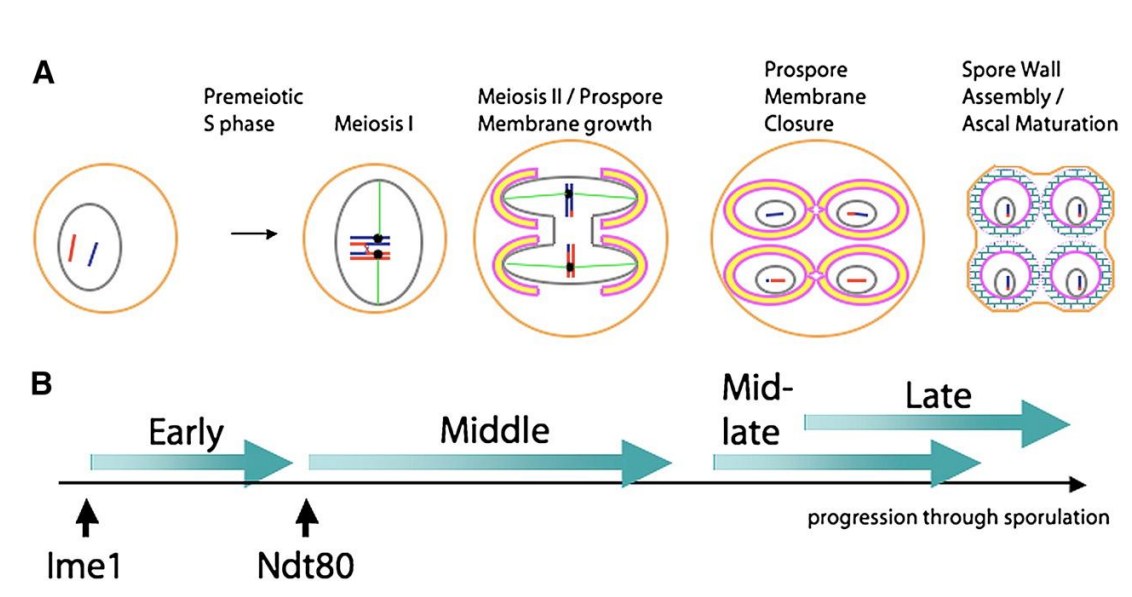
\includegraphics[width=0.55\textwidth]{images/sporlutation.png}
		\caption{A representation of the process of sporulation in budding yeasts}
		\label{fig:Sporlutation}
	\end{center}
\end{figure}


By utilizing DNA microarrays encompassing a significant portion of key genes, we can comprehensively investigate temporal gene expression patterns throughout the process of meiotic spore formation. However, this technique generates large datasets of unlabeled gene expression data, making pattern identification challenging. The abundance of expression levels for hundreds of genes at different time points presents an ideal scenario for applying clustering algorithms to uncover meaningful gene groups and understand the underlying transcriptional regulatory mechanisms.\cite{datta2003}

\subsection*{Application of Clustering Techniques to Analyze Sporulation Data}

While hierarchical clustering (UPGMA) with correlation distance has been a popular choice in microarray studies (at least the begginnings of this century), it's important to recognize the diverse range of clustering algorithms available in pattern recognition and statistics. To classify genes based on their temporal expression profiles during yeast sporulation, we will employ various clustering algorithms, including hierarchical clustering, K-means, self-organizing maps (SOM), and Diana. This comparative analysis aims to identify distinct gene expression patterns and gain insights into the underlying transcriptional regulatory mechanisms.\cite{datta2003}



\section{Description of the Methods}

There is a wide variety of clustering techniques, in this work it was decided to focus on details that were not carried out in the paper Comparisons and validation of statistical
clustering techniques for microarray gene
expression data by the Datta brothers, giving priority to the following:
\subsection{Clustering Techniques}


\begin{itemize}
	\item \textbf{Hierarchical Clustering:} is a method that groups data into a hierarchical structure rather than assigning a fixed number of clusters beforehand. It starts with each data point as a separate cluster and gradually merges the closest clusters until a single cluster remains.\cite{guess2002}
	
	\begin{itemize}
		\item \textbf{Algorithm:} The "average" method is used to calculate the distance between clusters. This method computes the average distance between points in one cluster and points in the other cluster.\cite{datta2003}
		
		\item \textbf{Common Method:} This approach, known as UPGMA, is a popular and straightforward method for hierarchical clustering.\cite{datta2003}
		
		\item \textbf{Distance Metric:} The distance between genes is calculated using a correlation-based measure, where a higher correlation indicates greater similarity between the gene expression profiles.\cite{datta2003}
	\end{itemize}
	
	
		
		\item \textbf{K-means:} is an unsupervised machine learning technique used to divide a dataset into distinct groups or clusters. Each cluster consists of data points that are more similar to each other than to those in other clusters. K-means is a popular clustering algorithm that partitions data into a predefined number of clusters, represented by centroids. The algorithm works iteratively to assign data points to the nearest centroid, updating centroids based on the mean of the points assigned to each cluster.\cite{steinley2006}
		
		\begin{enumerate}
			\item \textbf{Initialization:} k points are randomly selected from the dataset as initial centroids of the k clusters. These centroids represent the center of each cluster.
			\item \textbf{Assigning Points to Clusters:} Each data point is assigned to the cluster whose centroid is closest. The distance is usually calculated using the Euclidean distance.
			\item \textbf{Updating Centroids:} The positions of the centroids are recalculated as the average of all the points assigned to each cluster.
			\item \textbf{Repetition:} Steps 2 and 3 are repeated until the centroids no longer move significantly or a maximum number of iterations is reached.\cite{steinley2006}
		\end{enumerate}
		
		\item \textbf{Self-Organizing Maps (SOM):} is an unsupervised neural network that learns to map high-dimensional data onto a low-dimensional grid. It identifies representative prototype vectors and establishes a continuous mapping from the input space to this grid. The grid, often visualized as a 2D map (see Figure \ref{fig:som}), consists of neurons with associated weight vectors. These weight vectors are initially random but converge to represent clusters of similar data points during training.
		
	
\end{itemize}

\begin{figure}[h!]
	\begin{center}  % Usamos el entorno 'center'
		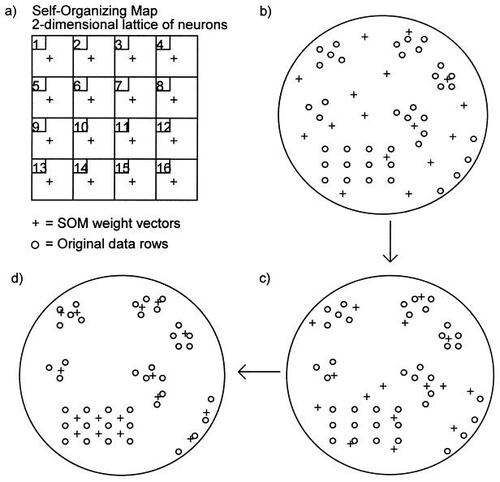
\includegraphics[width=0.45\textwidth]{images/som.jpg}
		\caption{The image illustrates the Self-Organizing Map (SOM) learning process. Panel (a) shows the initial SOM structure, (b) depicts the random initialization of weight vectors, (c) represents an intermediate stage of learning, and (d) shows the final configuration where weight vectors cluster around data points.}
		\label{fig:som}
	\end{center}
\end{figure}

\vspace{-30pt}

\subsection{Additional Clustering Methods which are theoretically mentioned}

\begin{itemize}
	\item \textbf{DIANA (Divisive Analysis Clustering):} This method differs from hierarchical clustering in that it starts with all data in a single cluster and progressively divides it into sub-clusters.\cite{datta2003}
	
	\item \textbf{Fanny:} Utilizes fuzzy logic to generate a probability vector for each observation, assigning observations to clusters based on the highest probability. L1 distance (Manhattan distance) is typically used as the dissimilarity measure, offering robustness compared to Euclidean distance. \cite{datta2003}
	
	\item \textbf{Model-based Clustering:} Treats the data as arising from a mixture of distributions, allowing for a probabilistic interpretation of clusters.\cite{datta2003}
	
	\item \textbf{Hierarchical Clustering with Partial Least Squares:} Leverages partial least squares to identify gene relationships through their expression profiles, demonstrating its effectiveness as noted by Datta (2001)\cite{datta2003}.
\end{itemize}

\subsection{Validation Methods}


To validate the obtained clusters, we can employ various strategies. One approach is to experiment with different numbers of clusters and observe how the average distance between points and their respective cluster centroids changes. This is known as the \textit{elbow method} due to the characteristic elbow shape of the resulting graph. However, the elbow method alone does not guarantee optimal cluster formation.\cite{Wang2018Thresher}

\subsubsection{Silhuoette}

To address this, we can utilize \textit{silhouette analysis}, a cluster validation technique based on the silhouette coefficient. The silhouette coefficient measures the similarity of a data point to its own cluster compared to its similarity to neighboring clusters. It ranges from -1 to 1, with values closer to 1 indicating better cluster membership and values closer to -1 suggesting misclassification.\cite{Wang2018Thresher}


In simple terms, it helps us determine whether the data has been grouped correctly and whether the clusters formed are coherent.
The silhouette coefficient is calculated as follows:

\begin{itemize}
	\item \(a\): The average distance between a point and all other points in its cluster. This tells us how well the point fits within its cluster.
	\item \(b\): The average distance between a point and all points in the nearest different cluster.This tells us how well the point would fit into the closest neighboring cluster.
\end{itemize}

\[
\text{Silhouette Coefficient} = \frac{(b - a)}{\max(a, b)}
\]

By calculating the average silhouette coefficient for all points within each cluster, we can assess the overall cluster validity. Combining silhouette analysis with the elbow method can help us determine the optimal number of clusters that minimize the overall distance between points and their clusters while maximizing the silhouette coefficient, suggesting well-formed and meaningful clusters.\cite{Wang2018Thresher}

\subsubsection{Calinski-Harabasz Index}


The Calinski-Harabasz Index (CHI) is a metric used to assess the quality of clustering in cluster analysis, offering a different approach from the silhouette coefficient. It evaluates the clustering performance by comparing two types of sum of squares:\cite{Ning2023Clustering}

\begin{itemize}
	\item \textbf{Between-cluster sum of squares (SSB):} Measures the separation between the cluster centroids. A higher SSB indicates that clusters are more distinct from each other.
	\item \textbf{Within-cluster sum of squares (SSW):} Measures the dispersion of data points within each cluster. A lower SSW indicates that the clusters are more compact.
\end{itemize}

The Calinski-Harabasz Index is calculated using the following formula:

\[
\text{CHI} = \frac{\text{SSB} / (k - 1)}{\text{SSW} / (n - k)}
\]

where:
\begin{itemize}
	\item $k$ is the number of clusters.
	\item $n$ is the total number of data points.
\end{itemize}

A higher CHI value indicates better clustering quality, as it suggests that clusters are well separated and the data within each cluster are homogeneous. Thus, the index provides a measure of the balance between cluster separation and the compactness of the data points within each cluster.\cite{Ning2023Clustering}

\subsubsection{The Davies-Bouldin Index}

 is a widely used metric for evaluating the quality of clustering, offering an approach that complements other measures such as the silhouette coefficient and the Calinski-Harabasz index. It provides an assessment of whether the formed clusters are both compact and well-separated. The index is calculated as the average similarity between each cluster and its most similar neighboring cluster, with lower values indicating better clustering performance.\cite{Davies1979Cluster}

\subsubsection*{Calculation of the Davies-Bouldin Index}

The computation of the DBI involves several steps:

\begin{enumerate}
	\item \textbf{Centroid Calculation:} For each cluster, compute the centroid, which is the average of all data points within the cluster.
	\item \textbf{Cluster Diameter Calculation:} For each cluster, calculate its diameter, defined as the maximum distance between any two points in the cluster.
	\item \textbf{Centroid Distance Calculation:} Calculate the distance between the centroids of each pair of clusters.
	\item \textbf{Similarity Calculation:} For each cluster, find the nearest neighboring cluster (the one with the closest centroid) and compute the similarity using the formula:
	\[
	S(i) = \frac{D(i) + D(j)}{d_{ij}}
	\]
	where:
	\begin{itemize}
		\item $S(i)$ is the similarity of cluster $i$ to its nearest neighbor $j$.
		\item $D(i)$ and $D(j)$ are the diameters of clusters $i$ and $j$, respectively.
		\item $d_{ij}$ is the distance between the centroids of clusters $i$ and $j$.
	\end{itemize}
\end{enumerate}

The Davies-Bouldin Index is then computed as the average of the similarity values for all clusters.\cite{Davies1979Cluster}

In essence, the Davies-Bouldin Index seeks to minimize the similarity between clusters, with lower values reflecting better-defined and more compact clusters.

\subsubsection{Average Proportion of Non-Overlap Measure} It is a metric used by the Datta brothers in Comparisons and validation of statistical clustering techniques for microarray gene expression data\cite{datta2003}, denoted as $V_1$, is used to evaluate the consistency of a clustering algorithm by examining the stability of gene assignments across different clustering scenarios. It is defined as:

\[
V_1 = \frac{1}{M l} \sum_{g=1}^{M} \sum_{i=1}^{l} \left( 1 - \frac{n(C_{g,i} \cap C_{g,0})}{n(C_{g,0})} \right),
\]

where:
\begin{itemize}
	\item $M$ is the total number of genes.
	\item $l$ is the number of time points.
	\item $C_{g,0}$ represents the cluster assignment of gene $g$ when using the full dataset.
	\item $C_{g,i}$ represents the cluster assignment of gene $g$ when the expression levels at time point $T_i$ are excluded.
	\item $n(C_{g,i} \cap C_{g,0})$ is the number of genes that remain in the same cluster in both the original and reduced datasets.
\end{itemize}

The measure calculates the average proportion of genes that are not assigned to the same cluster when comparing the clustering results obtained using the complete dataset with the results obtained after removing expression data for one time point. Lower values of $V_1$ indicate greater stability and consistency of the clustering algorithm, reflecting better preservation of gene cluster assignments despite variations in the data.\cite{datta2003}


\section{Data Analysis}

As mentioned, the dataset used in this study consists of gene expression data pertaining to the sporulation process in yeast (Saccharomyces cerevisiae), sourced from publicly available repositories and utilized in previous scientific research. To facilitate analysis, the data was processed using Python within the Google Colab environment.

As a preprocessing step, missing values, constituting 0.42\% of the dataset, were removed to ensure data integrity and consistency. Additionally, the data was standardized to mitigate the impact of varying data magnitudes on clustering algorithms like K-means.

To visualize gene expression patterns over time, the Python Seaborn library was employed. Heatmaps were generated to identify genes with similar temporal behavior and to detect any potential outliers or irregularities introduced during the standardization process.

Visual analysis revealed a stable distribution of data points across the variables, suggesting balanced representation and good standardization of the data. Notably, the variable t0 exerted a significant influence during bivariate analysis, consistently exhibiting a relatively stable proportion of examples in two distinct groups (refer to the first row and column of Figure \ref{fig:bivariante}). Moreover, t0 and T7 demonstrated a degree of stability in bivariate analysis with other variables. While a clear pattern is not immediately apparent for the remaining variables, it is premature to draw definitive conclusions, as complex interactions between variables may unveil hidden patterns upon further exploration. 

\begin{figure}[h!]
	\begin{center}  % Usamos el entorno 'center'
		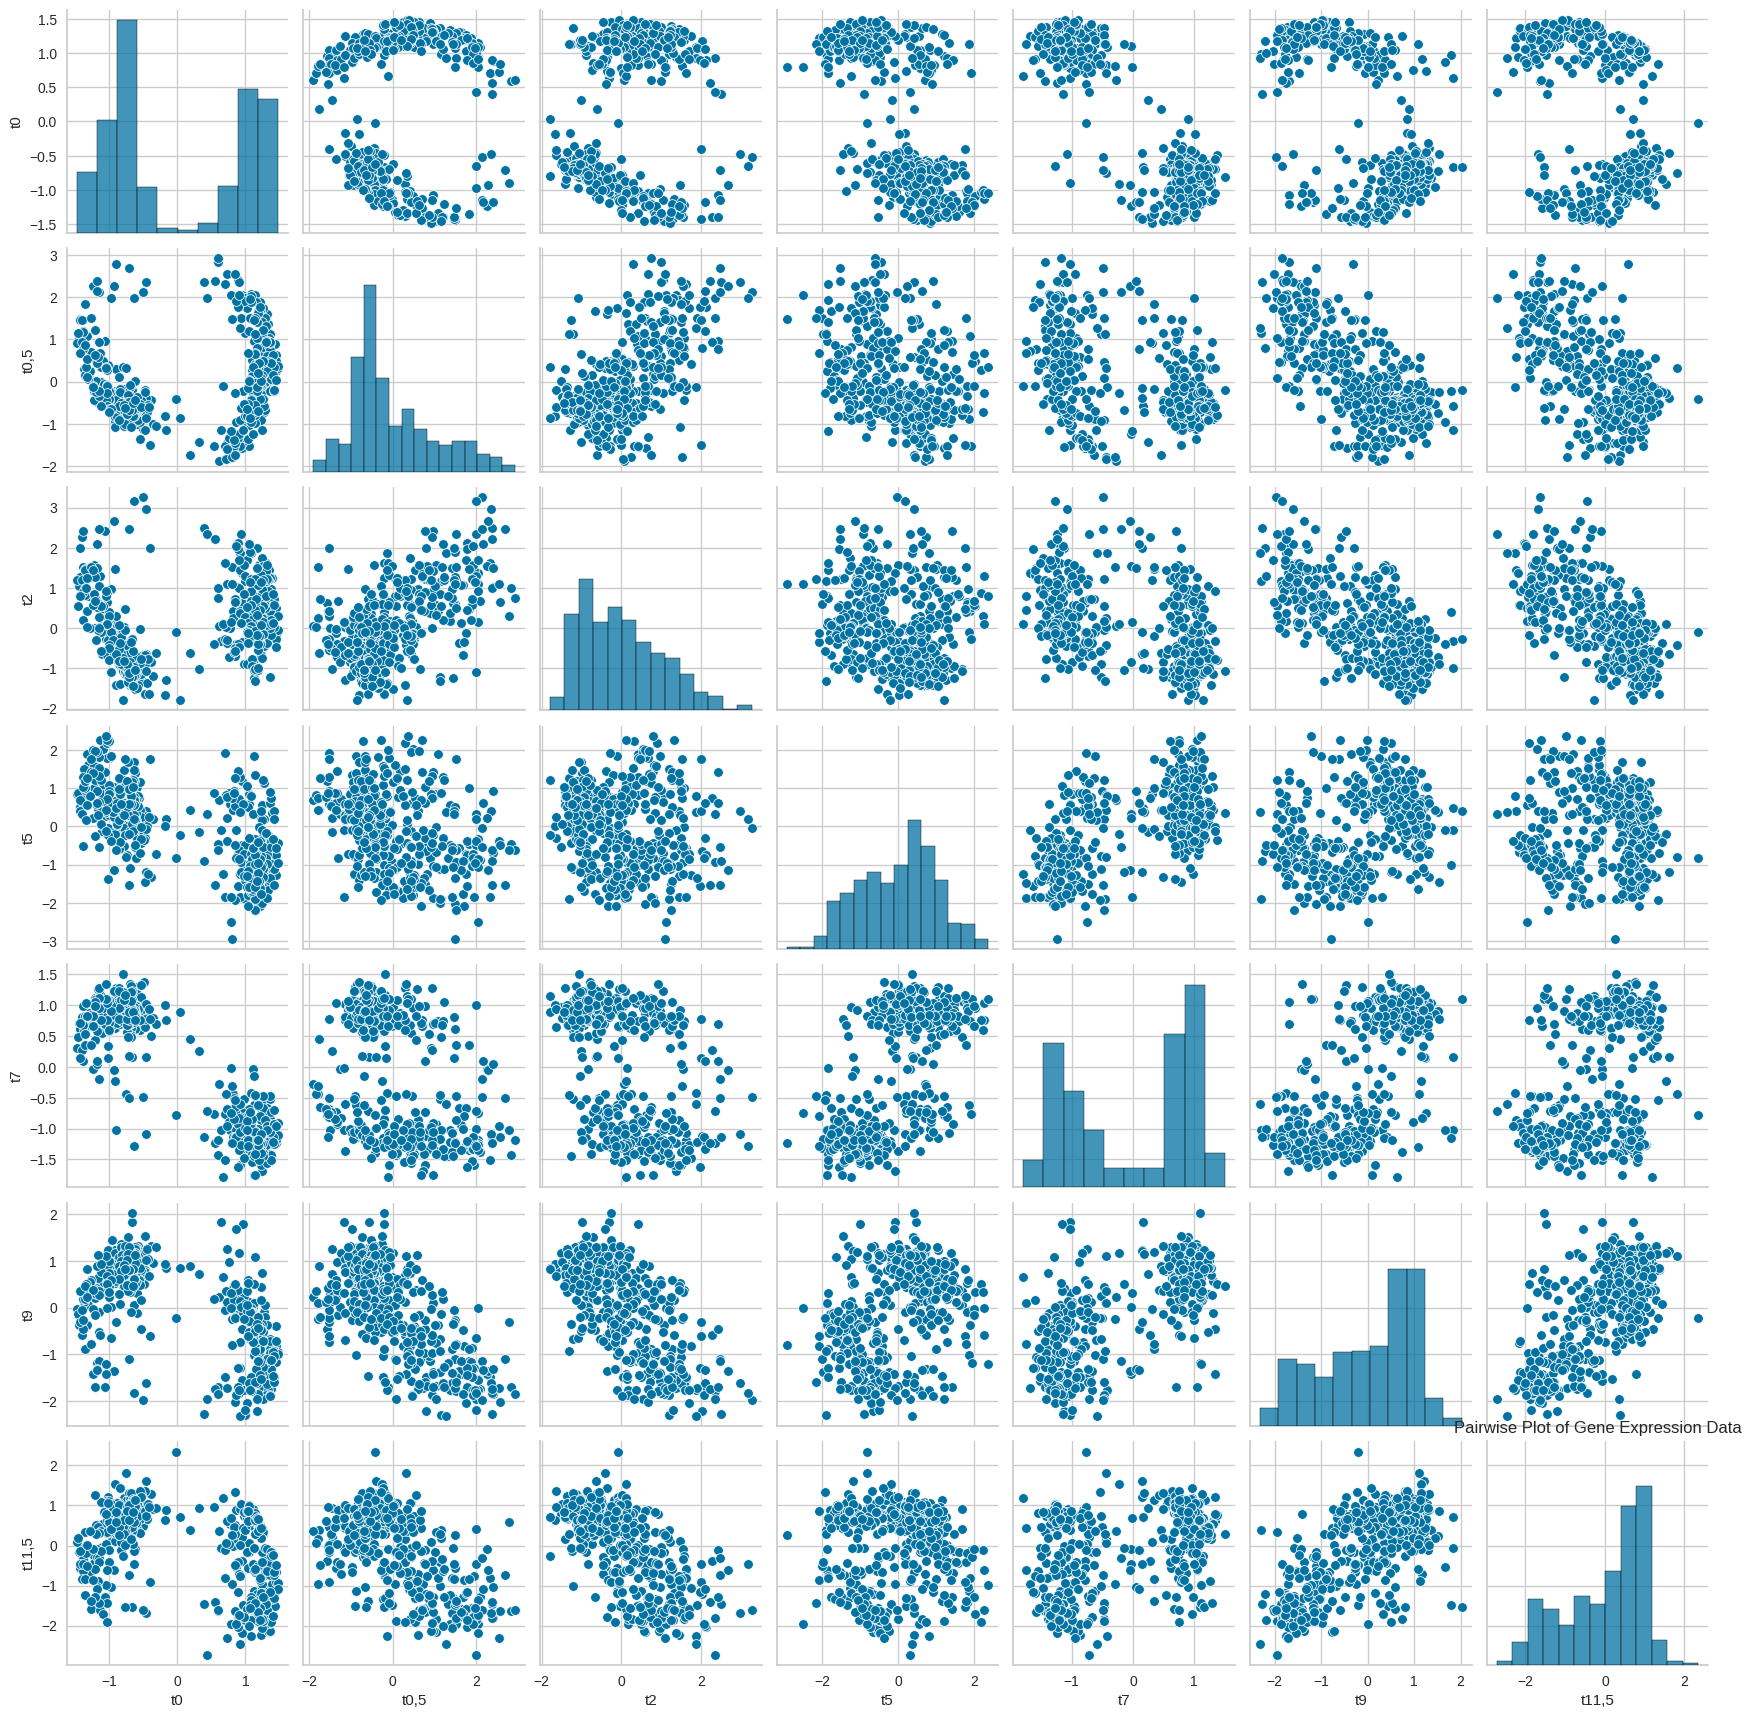
\includegraphics[width=0.75\textwidth]{images/Gene_Expression_Data.png}
		\caption{Scatter matrix of the variables in the dataset, generated with Seaborn. Each cell represents the relationship between two variables, showing their joint distribution and correlation.}
		\label{fig:bivariante}
	\end{center}
\end{figure}



\section{most relevant results}

A key focus of this study is to determine the optimal value for k when applying the K-means clustering algorithm. Additionally, we will compare the performance, advantages, and disadvantages of three clustering methods: K-means, hierarchical clustering, and self-organizing maps. To provide a broader context, we will also benchmark our results against the findings presented in the paper 'Comparisons and validation of statistical clustering techniques for microarray gene expression data' (May 2003), which utilized S+ for similar analyses.

\subsection{k-means}
 
 To determine the optimal K value for K-means clustering, multiple metrics were considered, with particular emphasis on the Silhouette Score and V1 (Average Proportion of Non-Overlap Measure). The Python scikit-learn library was employed to implement K-means and visualize the resulting metrics for K values ranging from 2 to 8 (Figure 4).
 
 While the elbow method suggested K = 4 as the optimal value, K = 2 consistently outperformed K = 4 in terms of the Silhouette Score and V1. These metrics indicate superior cluster separation and cohesion for K = 2, making it the preferred choice for this dataset.
 
 \begin{figure}[h!]
 	\begin{center}  % Usamos el entorno 'center'
 		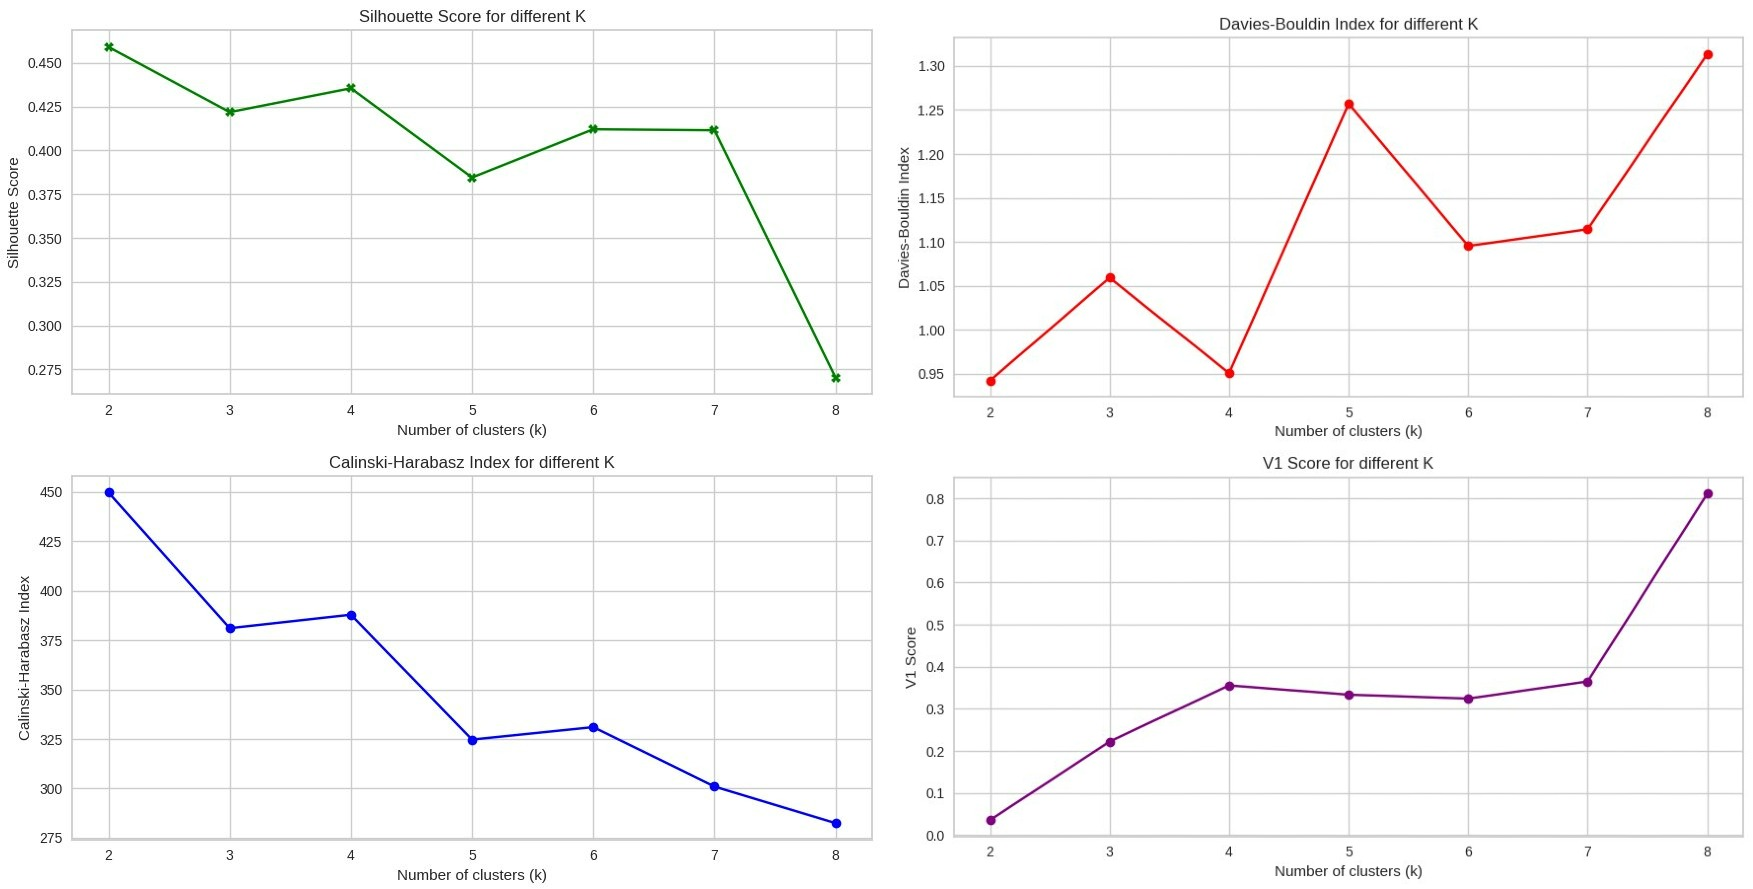
\includegraphics[width=0.9\textwidth]{images/kmeans.jpg}
 		\caption{Clustering metrics for K=2 to K=8: Silhouette Score, Davies-Bouldin Index, Calinski-Harabasz Index, and V1 Score.}
 		\label{fig:kmean}
 	\end{center}
 \end{figure}
 
 To address the complexity arising from the seven-dimensional dataset, the representation can become very complex, we employed Principal Component Analysis (PCA) as a dimensionality reduction technique. PCA transforms correlated variables into a smaller set of uncorrelated components, facilitating visualization and analysis. By applying PCA, we were able to project the data onto a 2D plane, enabling a more intuitive representation of the clustering results with the figure \ref{fig:kmean_representacion}.
 
  \begin{figure}[h!]
	\begin{center}  % Usamos el entorno 'center'
		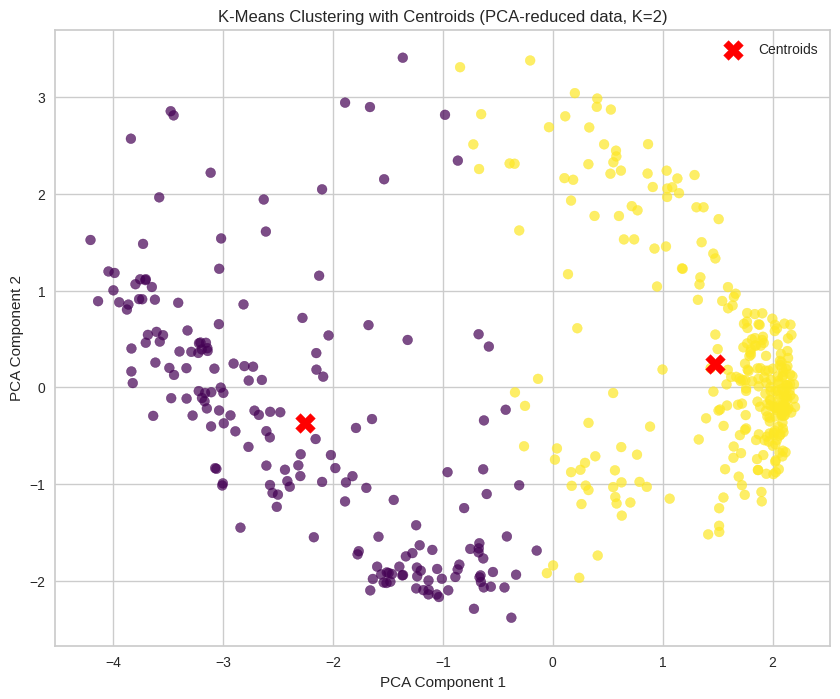
\includegraphics[width=0.5\textwidth]{images/kmeans_PCA_with_2_components_ k=2.png}
		\caption{Visualization of the dataset after dimension reduction with 2 cluster}
		\label{fig:kmean_representacion}
	\end{center}
\end{figure}
 
 As previously discussed, the Silhouette Coefficient is a valuable metric for evaluating cluster quality. In the case of K=2, we obtained a coefficient of 0.459. However, for a more comprehensive understanding, Figure \ref*{fig:kmean_silhoete} provides a visual representation of the silhouette scores for all data points within the two clusters. This visualization allows us to assess the distribution of silhouette values and identify any outliers or inconsistencies.In this analysis, we observe that certain data points are assigned to clusters that may not be their optimal fit. This is evident when examining the silhouette plot, where some points exhibit negative silhouette values, suggesting they might be better classified in alternative clusters.
 
 \begin{figure}[h!]
 	\begin{center}  % Usamos el entorno 'center'
 		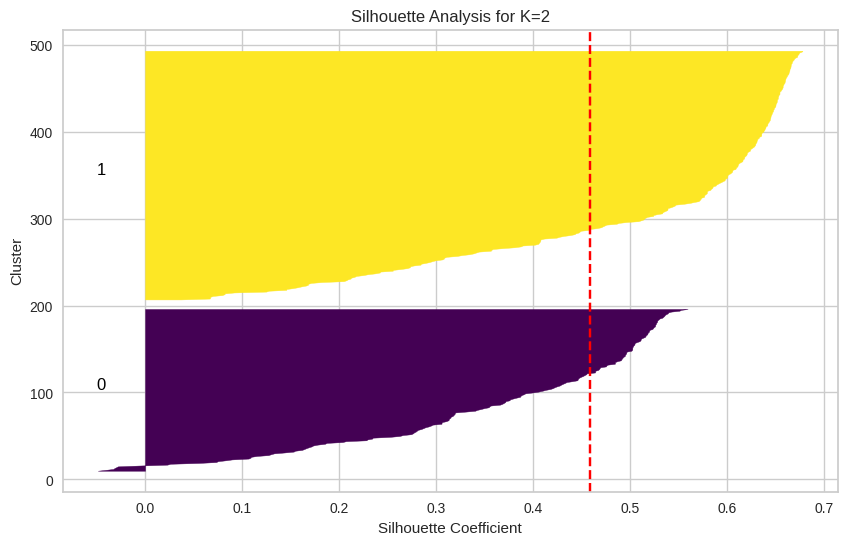
\includegraphics[width=0.75\textwidth]{images/silhouette_kmeans_PCA_with_2_components_ k=2.png}
 		\caption{Silhouette plot for K=2: Evaluating cluster cohesion and separation.}
 		\label{fig:kmean_silhoete}
 	\end{center}
 \end{figure}
 
 Although the possibility of a three-dimensional representation of the data was explored, it did not provide additional insights compared to two-dimensional visualization. The lack of clear separability between clusters in three-dimensional space, as well as the difficulty in visual interpretation, motivated the choice to discard these results.
 
 \subsection{Hierarchical Clustering (HC)}
 
Hierarchical clustering (HC) was implemented using the scikit-learn library to provide a complementary perspective to the K-means analysis. A dendrogram was constructed to visualize the hierarchical structure of the clusters and aid in interpreting the results. By examining the dendrogram and calculating relevant metrics, we were able to identify the optimal number of clusters.

The analysis of the figure \ref{fig:hyerarchical} revealed the formation of two unique clusters that encompass the entire dataset, aligning with the findings from the K-means clustering. However, the dendrogram also highlights the complex hierarchical relationships within the data. The tree-like structure illustrates how the data points are grouped at different levels of similarity. Lower branches represent more homogeneous subgroups, while higher branches indicate more heterogeneous clusters.

The complexity of the dendrogram reflects the inherent heterogeneity of the dataset, suggesting that while two primary clusters are evident, there may be finer-grained substructures within these clusters. Further exploration of these substructures could provide additional insights into the underlying patterns and relationships within the data.
 
 

  \begin{figure}[h!]
 	\begin{center}  % Usamos el entorno 'center'
 		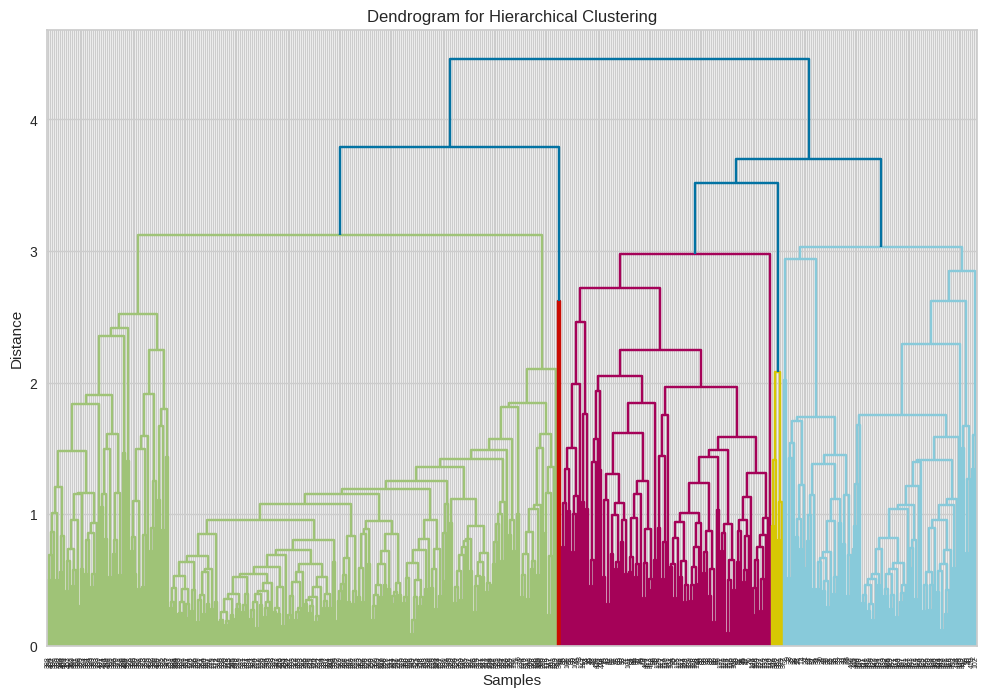
\includegraphics[width=0.45\textwidth]{images/hierarchical_clustering.png}
 		\caption{Hierarchical clustering (HC)}
 		\label{fig:hyerarchical}
 	\end{center}
 \end{figure}
 
  \subsection{Self-organizing maps (SOM)}
  
  While previous studies on this dataset have employed various clustering techniques, we chose to explore the application of Self-Organizing Maps (SOMs) using the minisom library in Python. Although SOMs can be a valuable tool, their performance is highly sensitive to parameters such as grid size, sigma value, learning rate, and thresholds.
  
  Our experiments with different SOM configurations revealed that the size of the map significantly influenced the clustering results. While larger maps (e.g., 25x25) might be expected to capture more complex patterns, we found that a smaller map size of 10x10 provided the most robust and meaningful clustering results (see the figure \ref{fig:SOM}), aligning with the conclusions drawn from other clustering methods.
  
  While SOMs can be effective, their performance can exhibit variability due to the inherent randomness in neural network training. In our experiments, SOMs generally yielded better results for the V1 metric and often suggested an optimal cluster number of 4, consistent with the elbow method. However, the overall performance of SOMs was relatively lower compared to K-means, indicating that K-means might be a more suitable choice for this particular dataset.
  
    \begin{figure}[h!]
  	\begin{center}  % Usamos el entorno 'center'
  		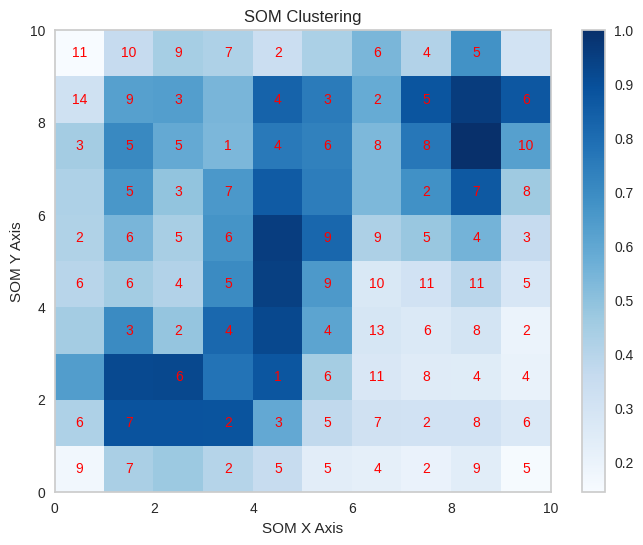
\includegraphics[width=0.45\textwidth]{images/SOM_clustering.png}
  		\caption{Hierarchical clustering (HC)}
  		\label{fig:SOM}
  	\end{center}
  \end{figure}
  
  \subsection{Comparative analysis of K-means, hierarchical clustering, and self-organizing maps}
  
  While clustering methods are essential for grouping data, comparing their performance can be challenging. The metrics employed in this study provide valuable insights into the relative strengths and weaknesses of each method. The following table \ref{tab:metrics_comparison} summarizes the key metrics and their corresponding values:
  
  \begin{table}[h!]
  	\centering
  	\begin{tabular}{|l|c|c|c|}
  		\hline
  		\textbf{Metric} & \textbf{K-Means (K=2)} & \textbf{Hierarchical} & \textbf{SOM} \\ \hline
  		\textbf{Calinski-Harabasz Index} & 449.800 & 398.349 & 86.597 \\ \hline
  		\textbf{Davies-Bouldin Index} & 0.942 & 1.002 & 1.192 \\ \hline
  		\textbf{Silhouette Score} & 0.459 & 0.439 & 0.151 \\ \hline
  		\textbf{V1 Score} & 0.036 & 0.014 & 0.335 \\ \hline
  	\end{tabular}
  	\caption{Comparison of clustering metrics across K-Means (K=2), Hierarchical Clustering, and SOM methods.}
  	\label{tab:metrics_comparison}
  \end{table}
  
  \begin{itemize}
  	\item \textbf{Calinski-Harabasz Index}: K-means exhibits the highest value, indicating superior cluster separation.
  	\item \textbf{Davies-Bouldin Index}: K-means also has the lowest value, suggesting compact and well-separated clusters.
  	\item \textbf{Silhouette Score}: K-means again outperforms the other methods, demonstrating well-defined clusters.
  	\item \textbf{V1 Score}: SOM shows the highest value, indicating greater stability when removing time points.
  \end{itemize}
  
  \textbf{Overall Assessment}:K-means (K=2) emerges as the preferred clustering method, demonstrating excellent performance across multiple metrics. While SOM excels in terms of stability, K-means offers a superior balance of cluster compactness, separation, and overall quality. Hierarchical clustering provides a reasonable alternative, but falls short in comparison to K-means.
  
  
  
  \subsection{Comparative with the paper "Comparisons and validation of statistical clustering techniques for microarray gene expression data"}
  
  Technological advancements, particularly in artificial intelligence, have accelerated rapidly. As a result, optimizing methodologies has become a paramount task for the growing community of programmers. Comparing technologies from different eras can be challenging due to significant advancements in both approaches and results.
  
  The paper 'Comparisons and validation of statistical clustering techniques for microarray gene expression data' (May 2002) utilized S+ for analysis. Despite the over two-decade difference in technology, this study demonstrates that the methods employed in the original paper may not yield identical performance when using Python-based tools. furthermore, although the dataset used is a Sporulation data microarray, the dataset used in the study reaches 6118 genes involved in total, a figure greater than the 474 genes used in this work.
  
  While the original study considered K values from 4 to 12, our analysis suggests that K=2 provides superior results in kmeans for the current dataset. Although the elbow method and SOM might favor K=4, K=2 consistently outperforms them in terms of the V1 metric and overall clustering quality when implemented kmean using Python's scikit-learn library.
 
 \section{Conclusions}
 
In this study, we conducted a comprehensive comparison of three clustering algorithms applied to a yeast sporulation dataset. The K-means algorithm, with K=2, demonstrated superior performance in terms of cluster compactness and separation, outperforming both hierarchical clustering and self-organizing maps. Nevertheless, each clustering method brings its own strengths and may perform better under different conditions or datasets. It is also crucial to consider the advancements in clustering methodologies and technology over time. By comparing our results to an older study, we observed that modern algorithms and computational power significantly enhance the quality of clustering outcomes, emphasizing the importance of continuous innovation in data analysis techniques.

\bibliographystyle{plain}  % Puedes cambiar "plain" por el estilo de tu preferencia, como apalike, ieeetr, etc.
\bibliography{bibliography}  % Aquí va el nombre de tu archivo .bib (sin la extensión .bib)
\end{document}
